\documentclass[10pt]{beamer}
\usepackage[utf8x]{inputenc}
\usepackage{hyperref}
\usepackage{fontawesome}
\usepackage{graphicx}
\usepackage{bm}

\usepackage{tikz}
\usepackage[english,ngerman]{babel}

\makeatletter
\newlength\beamerleftmargin
\setlength\beamerleftmargin{\Gm@lmargin}
\makeatother

% ------------------------------------------------------------------------------
% Use the beautiful metropolis beamer template
% ------------------------------------------------------------------------------
\usepackage[T1]{fontenc}
\usepackage{fontawesome}
\usepackage{FiraSans} 
\mode<presentation>
{
  \usetheme[progressbar=foot,numbering=fraction,background=light]{metropolis} 
  \usecolortheme{default} % or try albatross, beaver, crane, ...
  \usefonttheme{default}  % or try serif, structurebold, ...
  \setbeamertemplate{navigation symbols}{}
  \setbeamertemplate{caption}[numbered]
  %\setbeamertemplate{frame footer}{My custom footer}
} 

% ------------------------------------------------------------------------------
% beamer doesn't have texttt defined, but I usually want it anyway
% ------------------------------------------------------------------------------
\let\textttorig\texttt
\renewcommand<>{\texttt}[1]{%
  \only#2{\textttorig{#1}}%
}

% ------------------------------------------------------------------------------
% minted
% ------------------------------------------------------------------------------
\usepackage{minted}


% ------------------------------------------------------------------------------
% tcolorbox / tcblisting
% ------------------------------------------------------------------------------
\usepackage{xcolor}
\definecolor{codecolor}{HTML}{FFC300}

\usepackage{tcolorbox}
\tcbuselibrary{most,listingsutf8,minted}

\tcbset{tcbox width=auto,left=1mm,top=1mm,bottom=1mm,
right=1mm,boxsep=1mm,middle=1pt}

\newtcblisting{myr}[1]{colback=codecolor!5,colframe=codecolor!80!black,listing only, 
minted options={numbers=left, style=tcblatex,fontsize=\tiny,breaklines,autogobble,linenos,numbersep=3mm},
left=5mm,enhanced,
title=#1, fonttitle=\bfseries,
listing engine=minted,minted language=r}


% ------------------------------------------------------------------------------
% Listings
% ------------------------------------------------------------------------------
\definecolor{mygreen}{HTML}{37980D}
\definecolor{myblue}{HTML}{0D089F}
\definecolor{myred}{HTML}{98290D}

\usepackage{listings}

% the following is optional to configure custom highlighting
\lstdefinelanguage{XML}
{
  morestring=[b]",
  morecomment=[s]{<!--}{-->},
  morestring=[s]{>}{<},
  morekeywords={ref,xmlns,version,type,canonicalRef,metr,real,target}% list your attributes here
}

\lstdefinestyle{myxml}{
language=XML,
showspaces=false,
showtabs=false,
basicstyle=\ttfamily,
columns=fullflexible,
breaklines=true,
showstringspaces=false,
breakatwhitespace=true,
escapeinside={(*@}{@*)},
basicstyle=\color{mygreen}\ttfamily,%\footnotesize,
stringstyle=\color{myred},
commentstyle=\color{myblue}\upshape,
keywordstyle=\color{myblue}\bfseries,
}


% ------------------------------------------------------------------------------
% The Document
% ------------------------------------------------------------------------------
\title{Word vectors}
\author{Abe Handler, INFO 2301, CU Boulder}
\date{\today}

\begin{document}

\maketitle

\section{Word vectors}

\begin{frame}[fragile,allowframebreaks]{From words to math}
\begin{itemize}
\item{As humans, we usually take language for granted}
\item{I can talk to you on Zoom using a \textit{incredibly} complex symbolic system}
\item{By vocalizing certain sounds, I can put ideas in each of your heads}
\item{By vocalizing certain sounds, you can put ideas into my head}
\end{itemize}

\framebreak 
\begin{itemize}
\item{I say ``There is a quiz tomorrow'' and everyone understands what I mean}
\item{You say ``I am confused about scalar multiplication'' and I understand what you mean}
\item{You know the meaning of ``is'' and ``quiz'' and ``tomorrow'' and how to compose those words into a meaningful sentence}
\item{If I say ``I understands what you mean'' you can hear that I violated a grammar rule}
\end{itemize}

\framebreak 

This is all pretty amazing! Our brains just do this more or less automatically. It's not like dot product, where we have to take a class like 2301 to understand. 

\framebreak 

Unfortunately, computers don't have this easy facility with language. If you have ever used Siri or Alexa or been trapped in an automatic phone maze, you know that it's hard to get computers to understand human language. 

\begin{center}

\includegraphics[width=4cm]{siri.jpg}
\end{center}


\framebreak 

Word vectors are a technology for translating human language into math, something even a computer can understand

\framebreak 

Basic idea, each word gets a vector. Similar words are nearby in vector space.

\begin{center}
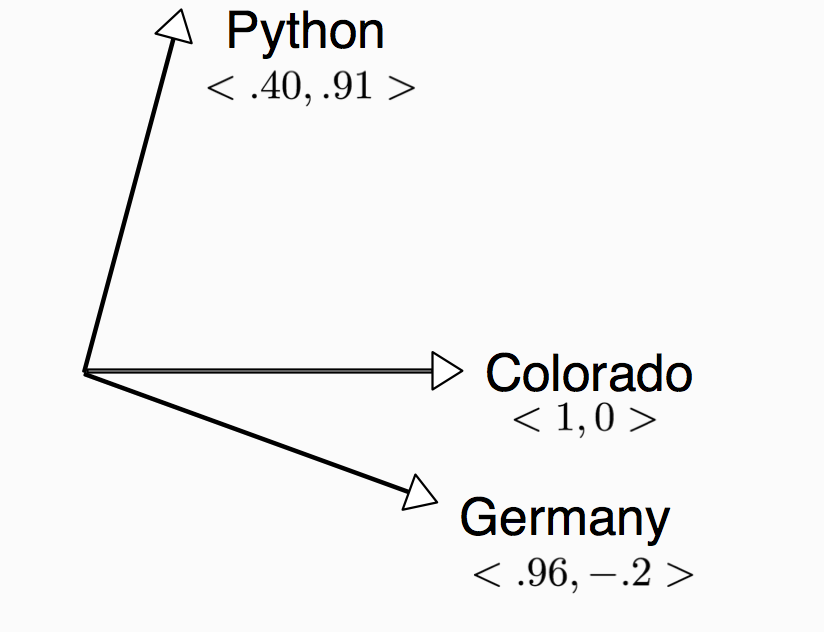
\includegraphics[width=4cm]{vecs.png}
\end{center}


\framebreak 

Notice that each vector in this example is normalized
\\ (i.e. magnitude = 1)

\\ Look at the vector for Germany, for instance. $.96^2 + -.2^2 =1$  \\
\\ (Well $\approx 1$ because of rounding)


\begin{center}
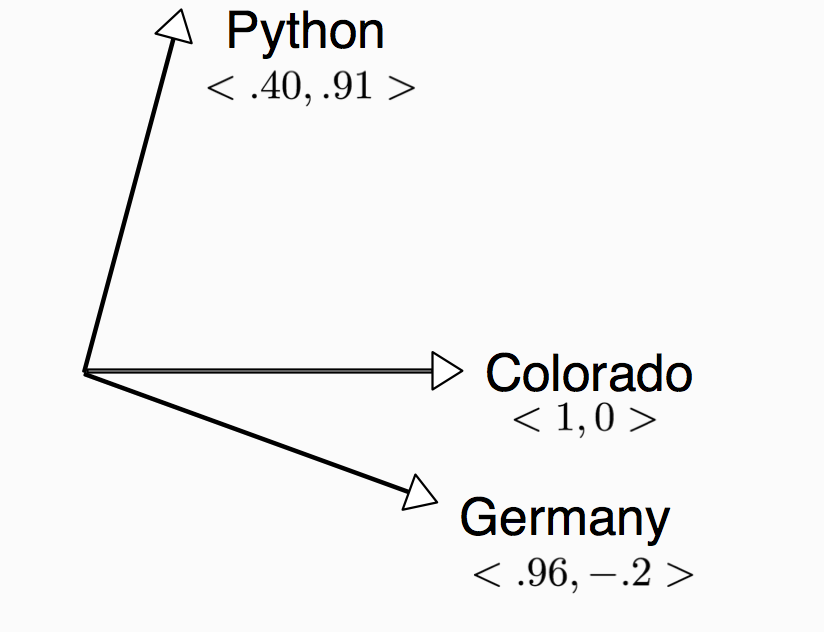
\includegraphics[width=4cm]{vecs.png}
\end{center}

\framebreak 

Which word is closer to Colorado? Germany? Or Python?

\begin{center}
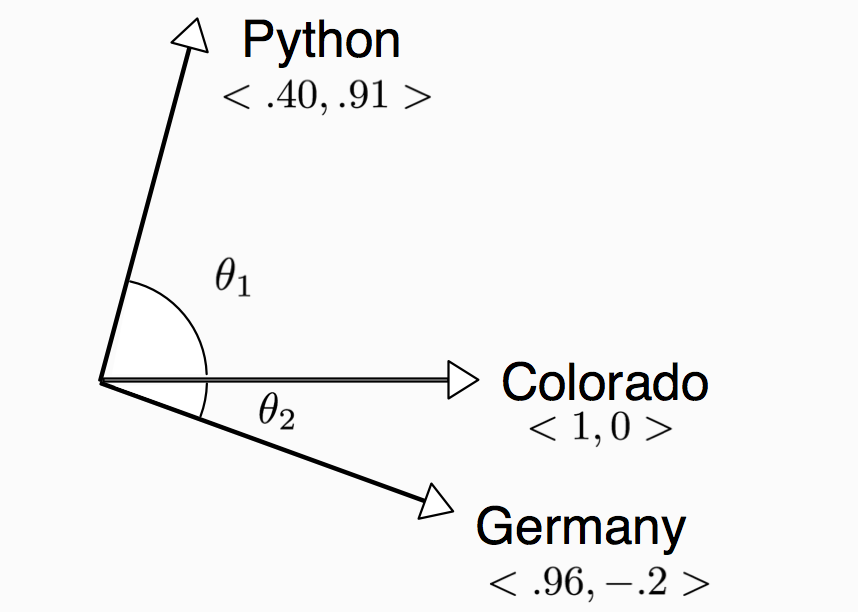
\includegraphics[width=4cm]{vecs2.png}
\end{center}

\framebreak 

Is $\theta_1$ or $\theta_2$ bigger?

\begin{center}
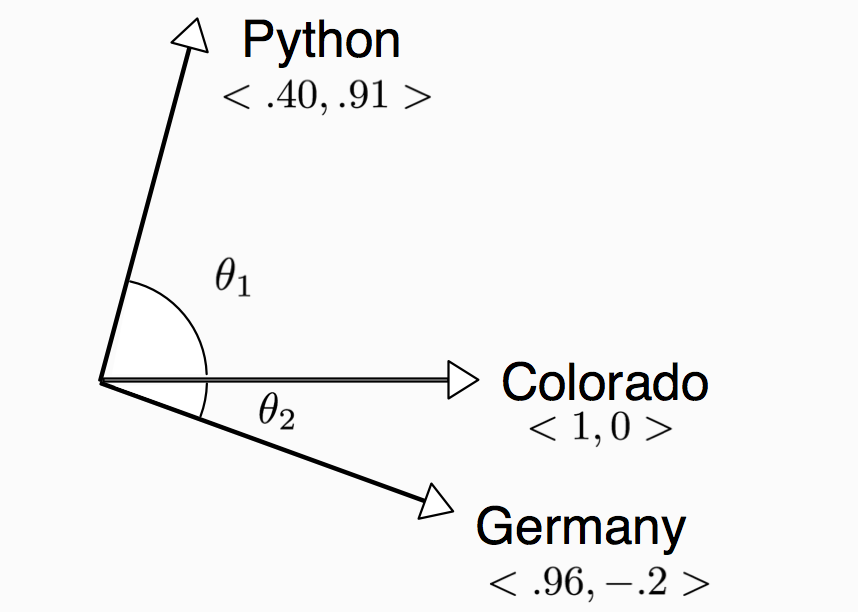
\includegraphics[width=4cm]{vecs2.png}
\end{center}

\framebreak 

Let $\bm{\hat{v}}_1$ = Python \\
Let $\bm{\hat{v}}_2$ = Colorado \\
Let $\bm{\hat{v}}_3$ = Germany

\begin{center}
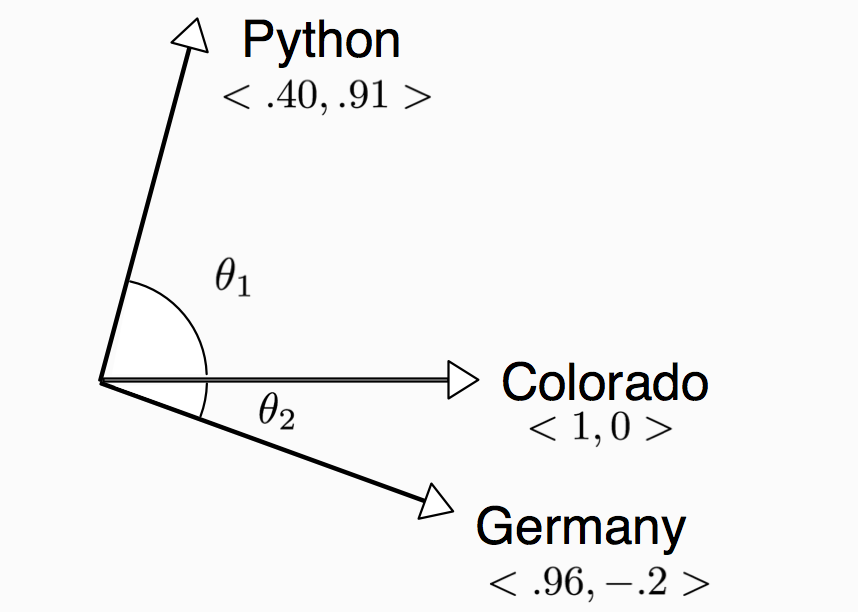
\includegraphics[width=4cm]{vecs2.png}
\end{center}


\framebreak 

Recall that $\bm{a} \cdot \bm{b} =  \lvert \lvert \bm{a}  \lvert \lvert * \lvert \lvert \bm{b}  \lvert \lvert  * \texttt{cos } \theta$  (Geometric definition)

Recall that $\bm{a} \cdot \bm{b} =  \Sigma a_i b_i$  (Algebraic definition)

\framebreak 

Python dot Colorado = ? \\

 Remember these are normalized unit vectors (e.g.\ $\lvert \lvert \bm{\hat{v}}_1  \lvert \lvert = 1$)\\ 
 
  $\bm{\hat{v}}_1 \cdot \bm{\hat{v}}_2 = \lvert \lvert \bm{\hat{v}}_1  \lvert \lvert * \lvert \lvert \bm{\hat{v}}_2  \lvert \lvert  * \texttt{cos} \theta_1 = 1 * 1 * \texttt{cos} \theta_1 =  \Sigma \bm{\hat{v}}_1 \bm{\hat{v}}_2 $  \\
 
\begin{center}
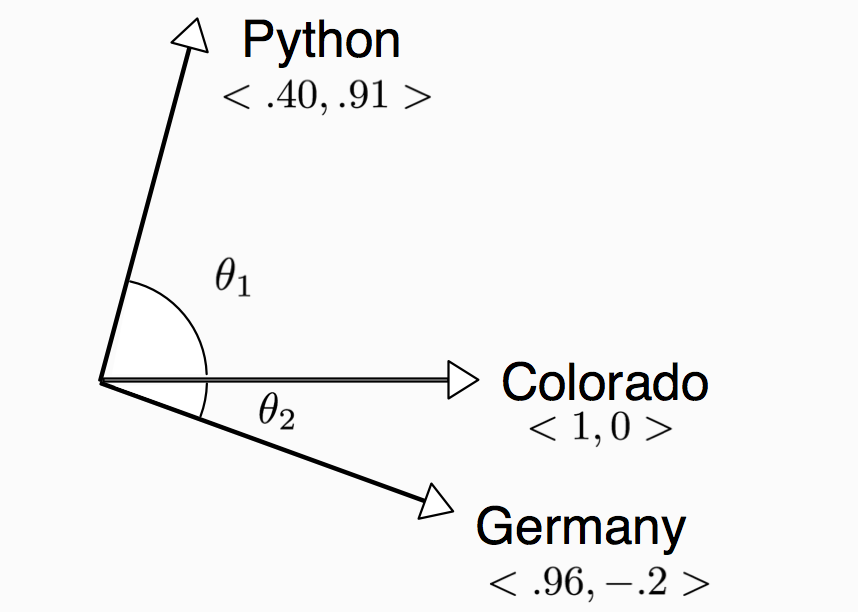
\includegraphics[width=4cm]{vecs2.png}
\end{center}

\framebreak 

Gemany dot Colorado = ? \\
 
  $\bm{\hat{v}}_2 \cdot \bm{\hat{v}}_3 = \lvert \lvert \bm{\hat{v}}_2  \lvert \lvert * \lvert \lvert \bm{\hat{v}}_3 \lvert \lvert  * \texttt{cos} \theta_2 = 1 * 1 * \texttt{cos} \theta_2 =  \Sigma \bm{\hat{v}}_2 \bm{\hat{v}}_3 $  \\
 
\begin{center}
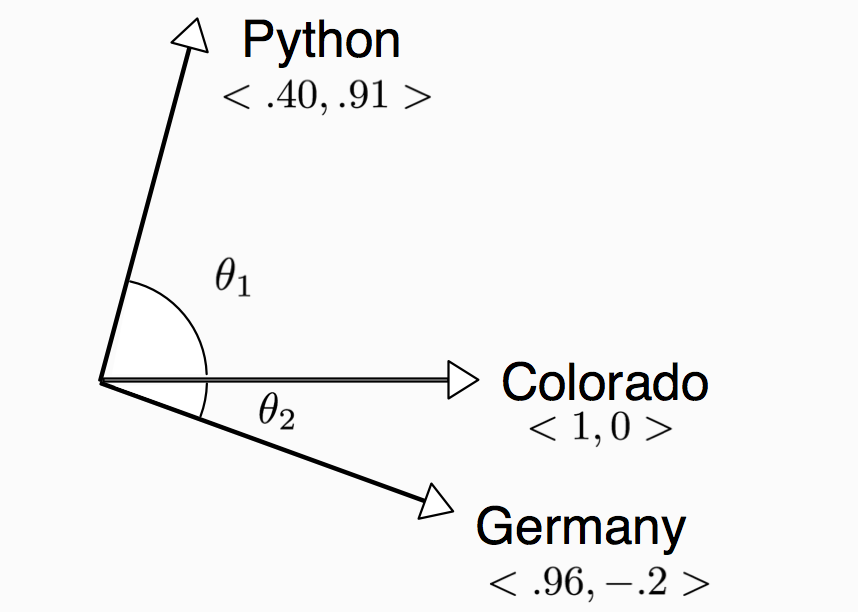
\includegraphics[width=4cm]{vecs2.png}
\end{center}

\end{frame}

\end{document}
